%-----------------------------------------------------------------
\setcounter{currentlevel}{\value{baseSectionLevel}}
\levelstay{Naive Sets}
\index{Set}
\epigraph{A pack of wolves, a bunch of grapes, or a flock of
pigeons are all examples of sets of things.
The mathematical concept of a set can be used as the foundation
for all known mathematics.
The purpose of this little book is to develop the basic properties
of sets.\\
\ldots \\
One thing that this development will not include is a definition
of sets.
The situation is analogous to the familiar axiomatic approach to
elementary geometry.
That approach does not offer a definition of points and lines;
instead it describes what it is that one can do with those
objects.
The semi-axiomatic point of view adopted here assumes that the
reader has the ordinary, human, intuitive (and frequently
erroneous) understanding of what sets are; the purpose of the
exposition is to delineate some of the things one can correctly do
with them.}%
{Halmos, \textit{Naive Set Theory}\cite{halmos_1960_naive_seth}}

\vfill

\emph{Sets} are a foundation for everything we are going to do,
but they turn out to be surprisingly hard to define precisely,
from first principles, without introducing paradoxes.

\vfill

\label{sec:math-sets}
\lstset{language=Clojure}

\cite{ferreiros2007labyrinth,sep-dedekind-foundations}

%-----------------------------------------------------------------
\setcounter{currentlevel}{\value{baseSectionLevel}-1}
\levelstay{Defining sets}
\epigraph{All the basic principles of set theory, except only the
axiom of extension, are designed to make new sets out of old ones.
The first and most important of these basic principles of set
manufacture says, roughly speaking, that anything intelligent one
can assert about the elements of a set specifies a subset, namely,
the subset of those elements about which the assertion is true.}
{Halmos, \textit{Naive Set Theory}~\cite[section~2]{halmos_1960_naive_seth}}

\begin{description}

\item[Specification]

A \gls{Set}, at its most fundamental, is a defined by a rule,
or method,
for determining if any given 'thing' is an element: 
$s \glssymbol{elementOf} \Set{S}$.
\footnote{$(s \notin \Set{S}) = \text{not}(s \in \Set{S})$.}
($s \not\in \Set{S}$)
%, or in pseudocode:
%\lstinline|(element-of $\Set{S}$ $s$)|.
An example, in standard set notation:
the even numbers 
$= \SetSpec{ i }{ \, i/2 \, \text{is an integer} }$.

\item[Enumeration]

However, it's difficult to do much interesting with a set
unless we have some way of finding, or generating elements.
So another common way to specify a set is by enumeration:
For example, the even numbers $= \{ \ldots, -4, -2, 0, 2 ,4,
\ldots \}$.

The enumeration notation above is something of a cheat ---
although it's straightforward enough for finite sets, it relies on
the reader correctly recognizing the implied pattern for countable
sets.
And it fails for uncountable sets like the real numbers.

\end{description}

What's unstated, but required, in both these approaches, is the
existence of some prior 'universe' set, $\Set{U}$, and a function
(see~\autoref{sec:Functions}) we can apply to the elements of
$\Set{U}$ to determine the set of interest:

\begin{description}
\item[Specification] 
$\Set{S} =
\SetSpec{ u \glssymbol{elementOf} \Set{U} }{ p(u) = \text{true} }$ 

For example: the even numbers
 $= \SetSpec{ i \glssymbol{elementOf} 
\glssymbol{Integers} }{
 i/2 \glssymbol{elementOf} \glssymbol{Integers} }$.

\item[Enumeration]
$\Set{S} =
\SetSpec{ f(u) }{ u \glssymbol{elementOf} \Set{U} }$ 

For example: the even numbers 
$= \SetSpec{ 2*i }{ i \glssymbol{elementOf} \glssymbol{Integers} }$.

\end{description}
A variation on 
``turtles all the way down''~\cite{xkcd:Turtles, wiki:Turtles},
this approach may be a bit unsatisfying.
It does, however, have the advantage of preventing self-reference
paradoxes (for example, 
the set of all sets that do not contain themselves); 
see Halmos, 
\textit{Naive Set Theory}~\cite[section 2]{halmos_1960_naive_seth} 
for details.

% \gls{empty set}
One set that doesn't require any turtles is 
the empty set, $\varnothing$.


Both approaches raise the fascinating issue of 
computability/decidability~\cite{church1936unsolvable,
turing1936computability,
turing1938computable-correction,
turing1937computability-lambda},
which I am going to pass over here, except to note the 
'halting problem'~\cite{wiki:Halting-problem}:

If we call $p(u)$ to determine if $u \in \Set{S}$, 
it might return $\text{true}$, might return $\text{false}$,
or it might not return at all.
In the third case, we might define $u \in \Set{S}$ as only those
$u$ where $p(u)$ halts and returns $\text{true}$, but it turns 
out that given $p$ and $u$, deciding whether $p(u)$ will ever
finish is itself undecidable (more turtles \ldots).

The practical version of this is that, even in cases where we
might be able to determine that $p(u)$ that will eventually halt
and return something, we might not be able to afford to wait that
long.
Pragmatically, we will have to restrict ourselves to sets where we
can guarantee an answer fast enough for the context in which the
sets are being used.

%-----------------------------------------------------------------
\setcounter{currentlevel}{\value{baseSectionLevel}-1}
\levelstay{Cardinality}

% \gls{cardinality}  \gls{countable infinity} \gls{uncountable
% infinity} \gls{cardinal numbers}
The cardinality of a set in the number of elements.
For our purposes, the possibilities that matter are \emph{finite,}
\emph{countably infinite}, the cardinality of the
\gls{NaturalNumbers}, $\aleph_{0}$, or \emph{uncountably
infinite}, which means the set has more elements than the
\gls{NaturalNumbers}.
(I'm ignoring the distinction between different uncountable
infinities.
See~\cite{wiki:cardinal-number} for an introduction to the other
possibilities.)

Notation for set cardinality varies widely:
$\#\Set{S}$,  $|\Set{S}|$,
$\bar{\bar{\Set{S}}}$, $n(\Set{S})$,
$\text{card}(\Set{S})$, \ldots, nearly all of which conflict
with something (eg $\#\{ 0 \, 1 \, 2 \} = 3$ vs 
\lstinline|#{1 2 3}| Clojure set syntax).
I will use $\text{cardinality}(\Set{S})$.

%-----------------------------------------------------------------
\setcounter{currentlevel}{\value{baseSectionLevel}-1}
\levelstay{Identity}

The question of whether two sets are the same set is a recurring
locus of ambiguity in mathematics.

One issue is the difference between the 'set' and the 
'set definition', which is rarely made clear.

Halmos~\cite{halmos_1960_naive_seth} starts with the \emph{Axiom of
extension:} two sets are the \emph{same thing} if they have the
same elements (regardless of how they are defined).

Example: 
$\SetSpec{ 2*i }{ \, i \in \glssymbol{Integers} }$
and
$\SetSpec{ i \in \glssymbol{Integers} }
{ i/2 \in \glssymbol{Integers} }$
are two distinct definitions of the same set. 
 
Pragmatically, however, it's going to be much easier to determine
if two set definitions are the same, than determining if two
different definitions generate the same elements, which would,
after all, be undecidable in general.

Another source of ambiguity is a common tendency to blur the 
distinction between sets whose elements are related by some natural
identity. 

Example: we can define the rational numbers as (equivalence
classes of) pairs of integers:
$\glssymbol{RationalNumbers} = \glsdesc{RationalNumbers}$.
Strictly speaking, the rational number $i/1$ is a different thing
from the integer $i$, but it's nearly universal to identify the
subset of the rationals with denominator $1$ with the integers and
take $\glssymbol{Integers} \subset \glssymbol{RationalNumbers}$.

%-----------------------------------------------------------------
\setcounter{currentlevel}{\value{baseSectionLevel}-1}
\levelstay{Subsets, partitions, and quotients}

Families: 
$\SetSpec{ \Set{S}_{i} }{ i \in \, \text{index set} \, \Set{I} }$.


%\gls{subset} \gls{superset}

$\Set{A} \subseteq \Set{B}$ ($\Set{B} \supseteq \Set{A}$)
means
every element of $\Set{A}$ is an element of $\Set{B}$, 
that is, $a \in \Set{A}$ 
implies $a \in \Set{B}$.
I reserve $\Set{A} \subset \Set{B}$ (($\Set{B} \supset
\Set{A}$)) for strict subsets;
it means $\Set{A} \subseteq \Set{B}$
and there is some $\b\in\Set{B}$ which
is not in $\Set{A}$.

%\gls{power set}

The \emph{power set}, $\PowerSet{\Set{S}}$,
 is the set 
of all subsets of
$\Set{S}$.

%\gls{intersection} \gls{union} \gls{set-difference}
As usual, $\Set{A} \cap \Set{B}$ is the set of elements in both 
$\Set{A}$ and $\Set{B}$; $\Set{A} \cup \Set{B}$ are those things
that are in either $\Set{A}$ or $\Set{B}$.

$\Set{A} \cap \Set{B} \cap \Set{C} 
= (\Set{A} \cap \Set{B}) \cap \Set{C} 
= \Set{A} \cap (\Set{B} \cap \Set{C}) $

$\bigcap_{i \in \Set{I}} \Set{S}_{i} = 
\SetSpec{ s }{ s \in \Set{S}_{i} \forall \Set{S}_{i} }$

$\Set{A} \setminus \Set{B}$ are the elements of $\Set{A}$ 
not in $\Set{B}$.

%\gls{partition}
A partition of $\Set{S}$ is a set of disjoint nonempty subsets of
$\Set{S}$ whose union is $\Set{S}$.

%-----------------------------------------------------------------
\setcounter{currentlevel}{\value{baseSectionLevel}-1}
\levelstay{Implementation}

%-----------------------------------------------------------------
\setcounter{currentlevel}{\value{baseSectionLevel}-2}
\levelstay{Java}
\lstset{language=Java}

Java provides an interface \lstinline|java.util.Set| intended for
possibly mutable, finite sets (\autoref{java.util.Set:general},
 \autoref{java.util.Set:countable}, 
 \autoref{java.util.Set:finite}, 
 and
\autoref{java.util.Set:optional}).

%-----------------------------------------------------------------
\begin{lstlisting}[
 caption={[\texttt{java.util.Set} general]\texttt{java.util.Set} 
 operations applicable to any set.}, 
 label=java.util.Set:general]
boolean contains (Object o) //$ \; o \in \Set{S}$
boolean containsAll (Collection c) //$\;\Set{C}\subseteq\Set{S}$ 
boolean isEmpty () //$ \; \Set{S} = \varnothing $
boolean equals (Object o) //$\; \Set{S} = \Set{O} $
\end{lstlisting}
%-----------------------------------------------------------------
\begin{lstlisting}[
 caption={[\texttt{java.util.Set} countable]\texttt{java.util.Set} 
 operations requiring countable sets. Note, however, that 
 iterators that never end will cause havoc with almost all Java
 code}, 
 label=java.util.Set:countable]
Iterator iterator ()
Spliterator spliterator ()
\end{lstlisting}
%-----------------------------------------------------------------
\begin{lstlisting}[
 caption={[\texttt{java.util.Set} finite]\texttt{java.util.Set} 
 operations requiring finite sets. Note that changing to
 \texttt{size()} to be Object valued would enable representing sets
 of arbitrary cardinality.}, 
 label=java.util.Set:finite] 
int size () 
Object[] toArray ()
Object[] toArray (Object[] a)
\end{lstlisting}
%-----------------------------------------------------------------
\begin{lstlisting}[
 caption={[\texttt{java.util.Set}]\texttt{java.util.Set} optional
 operations, requiring mutable sets.}, 
 label=java.util.Set:optional,]
boolean add(E e) //$\; \Set{S} \leftarrow \Set{S} \cup \{e\} $
boolean addAll(Collection c) //$\;\Set{S}\leftarrow\Set{S}\cup\Set{C}$ 
void  clear() //$\; \Set{S} \leftarrow \varnothing $ 
boolean remove (Object o) //$\;\Set{S}\leftarrow\Set{S}\setminus\{e\}$
boolean removeAll (Collection c) //$\;\Set{S}\leftarrow\Set{S}\setminus\Set{C}$ 
boolean retainAll (Collection c) //$\;\Set{S}\leftarrow\Set{S}\cap\Set{C}$
\end{lstlisting}
%-----------------------------------------------------------------

More Java set classes? Guava or Apache Commons?
Set operations, union, cartesian products, \ldots.

%-----------------------------------------------------------------
\setcounter{currentlevel}{\value{baseSectionLevel}-2}
\levelstay{Clojure}
\lstset{language=Clojure}

Idiomatic Clojure sets are immutable, although it provides easy
access to any mutable or immutable Java implementation of
\lstinline|java.util.Set|.

Clojure provides an (unfortunate) literal syntax for finite
enumerated sets: 
\lstinline|#{0 1 2}|, and 4 ways to create sets:
\begin{description}
\item[\texttt{hash-set}] A function equivalent to the
literal syntax \lstinline|#{}|
\item[\texttt{sorted-set}/\texttt{sorted-set-by}] Returns
sets that iterate over their elements in their natural order (in the
order of the supplied comparator). Like Java sorted collections,
can't handle partial orderings.
\item[\texttt{set}] Coerce any collection into a set.
\item[\texttt{into}] A general way to coerce any collection
into another type.
\end{description}

Idiomatic Clojure provides an informally specified functional
'API' for finite sets. Most of these functions do will something
for all Clojure collections, not always what you would expect:
\begin{lstlisting}[
 caption={Clojure set 'API'}, 
 label=Clojure:set-API,]
(contains? s x) ;;  $x \in \Set{S}$.
(empty? s) ;; $\Set{S} = \varnothing$
(count s) ;; $\text{cardinality}(\Set{S})$
(conj s x) ;; $\Set{S} \cup \{x\}$
(disj s x) ;; $\Set{S} \setminus \{x\}$
(clojure.set/intersection s0 s1 s2 $\ldots$) ;; $\Set{S}_0 \cap \Set{S}_1 \cap \Set{S}_2 \cap \ldots$ 
(clojure.set/union s0 s1 s2 $\ldots$) ;; $\Set{S}_0 \cup \Set{S}_1 \cup \Set{S}_2 \cup \ldots$ 
(clojure.set/difference s0 s1 s2 $\ldots$) ;; $\Set{S}_0 \setminus (\Set{S}_1 \cup \Set{S}_2 \cup \ldots)$
\end{lstlisting}

Confusion with dictionary 'API':
 \lstinline|(s x)| and \lstinline|(get s x)| are similar to
 \lstinline|(contains? s x)| except \lstinline|(contains? s x)| returns
 \lstinline|true| or \lstinline|false|, while the other two return
 \lstinline|x| if \lstinline|x| is in \lstinline|s| \lstinline|nil| otherwise.
The behavior of \lstinline|(s x)| and \lstinline|(get s x)| reflect an
incomplete/inconsistent API treating Clojure collections as
dictionaries (key-value pairs), modeling sets as dictionaries
where the key and value are constrained to be the same.
However, other functions designed for dictionaries (eg
\lstinline|keys|) don't work for sets.
 
%-----------------------------------------------------------------
\setcounter{currentlevel}{\value{baseSectionLevel}-2}
\levelstay{Les Elemens}

Set interface.

Implementation almost always requires multiple objects
representing a single set element

\begin{equation}
a \parallel b
\end{equation}
vs
\begin{equation}
a = b
\end{equation}

vs
\begin{equation}
a \equiv b
\end{equation}

% \begin{lstlisting}[
% caption={[checksum namespace]Checksum and related functions via
% Java calls}, label=checksum-namespace,]
% (set! *warn-on-reflection* true)
% (set! *unchecked-math* :warn-on-boxed)
% (ns ^{:doc "compute a file checksum."}
%   
%   curate.scripts.checksum
%   
%   (:require [clojure.java.io :as io])
%   (:use [clojure.set :only [difference]])
%   (:gen-class))
% ;;-----------------------------------------------------------------
% (defn checksum [file]
%   (let [input (java.io.FileInputStream. file)
%         digest (java.security.MessageDigest/getInstance "MD5")
%         stream (java.security.DigestInputStream. input digest)
%         bufsize (* 1024 1024)
%         buf (byte-array bufsize)]
% 
%   (while (not= -1 (.read stream buf 0 bufsize)))
%   (apply str (map (partial format "%02x") (.digest digest)))))
% 
% (defn list-dir [dir]
%   (remove #(.isDirectory %)
%           (file-seq (java.io.File. dir))))
% 
% (defn find-dupes [root]
%   (let [files (list-dir root)]
%     (let [summed (zipmap (pmap #(checksum %) files) files)]
%       (difference
%        (into #{} files)
%        (into #{} (vals summed))))))
% 
% (defn remove-dupes [files]
%   (prn "Duplicates files to be removed:")
%   (doseq [f files] (prn (.toString f)))
%   (prn "Delete files? [y/n]:")
%   (if-let [choice (= (read-line) "y")]
%     (doseq [f files] (.delete f))))
% 
% (defn -main [& args]
%   (if (empty? args)
%     (println "Enter a root directory")
%     (remove-dupes (find-dupes (first args))))
%   (System/exit 0))
% \end{lstlisting}
% 
% \lstinputlisting[
% float=htbp,
% caption={[checksum function]Compute a checksum for a file thru Java},
% label=checksum,
% firstline=11,lastline=18]{listings/checksum.clj}
 
%-----------------------------------------------------------------
\setcounter{currentlevel}{\value{baseSectionLevel}-1}
\levelstay{Examples}
 
1d and 2d intervals.
 
% \begin{minipage}{\linewidth}
% \begin{lstlisting}[
% caption={[FileTypeFilter]A file .suffix filter},
% label=FileTypeFilter]
% package img;
% 
% public final class FileTypeFilter 
%   implements java.io.FilenameFilter {
% 
%   private final String _suffix;
% 
%   public final boolean accept (final java.io.File dir,
%                                final String name) {
%     return name.toLowerCase().endsWith(_suffix); }
% 
%   public FileTypeFilter (final String suffix) {
%     super();
%     _suffix = suffix.toLowerCase(); } }
% \end{lstlisting}
% \end{minipage}
% 
% \index{Sets|)}
% 
% \begin{figure}[htbp]
% \centering
% 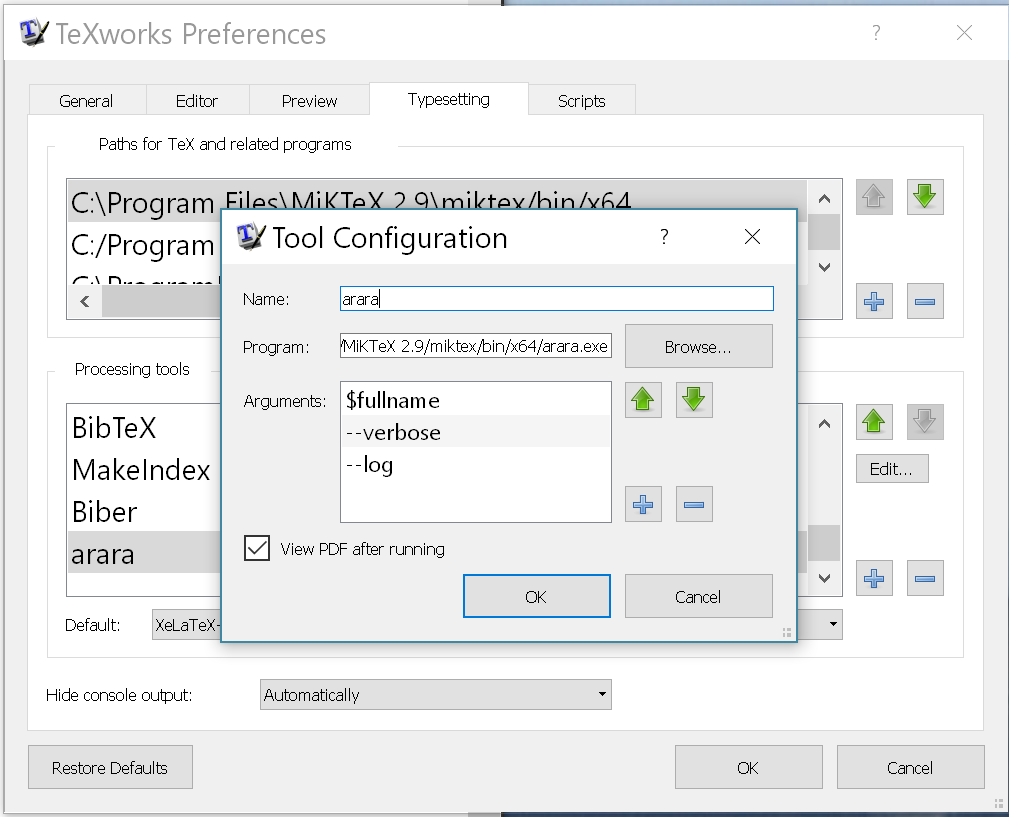
\includegraphics[scale=0.7]{figs/arara.png}
% \caption{Configuring {\TeX}works for \texttt{arara}.}
% \end{figure}
%-----------------------------------------------------------------
%-----------------------------------------------------------------
%-----------------------------------------------------------------
\setcounter{currentlevel}{\value{baseSectionLevel}}
\levelstay{Paradoxes}
\label{sec:Paradoxes}

Russell paradox~\cite{iep:Russell_paradox}

Russell-Myhill paradox(\cite{iep:Russell_Myhill_paradox})

%-----------------------------------------------------------------
%-----------------------------------------------------------------
%-----------------------------------------------------------------
%-----------------------------------------------------------------
\setcounter{currentlevel}{\value{baseSectionLevel}}
\levelstay{Set theories}


Axiomatic theories of various kinds.
Notes almost entirely from 
Wikipedia\cite{wiki:Set_theory,iep:Set_theory,eom:Set_theory,sep:Set_theory}.

\setcounter{currentlevel}{\value{currentlevel}-1}
%-----------------------------------------------------------------
%-----------------------------------------------------------------
%-----------------------------------------------------------------
\levelstay{Cantor set theory}
\label{sec:Cantor_set_theory}

``In his development of set theory, 
Cantor identified a single fundamental principle, 
called the Comprehension Principle, 
under which one can form a set.
Cantor’s principle states that, 
given any specific property $\varphi(x)$ 
concerning a variable $x$, 
the collection $\{x:\varphi(x)\}$ is a set, 
where $\{x:\varphi(x)\}$ is 
the set of all objects x that satisfy the property φ(x).
For example, let $\varphi(x)$ be the property that 
'$x$ is an odd natural number.' 
The Comprehension Principle implies that

$\Set{S}=\{x:\varphi(x)\}=\{1,3,5,7,\dots\}$ ``\cite{iep:Set_theory}

Problems: \hfill\break
where do we get the $x$ to plug into $\varphi(x)$?\hfill\break
if $x\in\mathbb{N}$, I think I know how to tell if it's odd;
how do I verify $x\in\mathbb{N}$,?\hfill\break
what does ``\dots'' mean?\hfill\break
what is $\varphi$ exactly?\hfill\break
if $\varphi$ is ``computable'' in some sense,
then it might return true, or return false, or not return
(infinite loop or recursion). what happens then?

%-----------------------------------------------------------------
%-----------------------------------------------------------------
%-----------------------------------------------------------------
\levelstay{von Neumann universe}
\label{sec:von_Neumann_universe}

Attributed to von Neumann, but may really be due to
Zermelo\cite{Zermelo:1930:ZERBGU}.

von Neumann universe: \textsf{V}\cite{wiki:Von_Neumann_universe},
the class of hereditary well-founded sets.

Hereditary set: elements are all hereditary sets, 
starting from empty set\cite{wiki:Hereditary-set}.

All elements of sets are sets themselves.

No \textsl{ur-elements}\cite{wiki_2020_urelement} 
(aka ``atoms'', ``individuals'') ---
non-set things that may belong to a set.

(Note: \textsl{proper class} is dual to ur-element in the sense that
ur-elements do not have elements and proper classes cannot be 
elements.)

(Perhaps elegant---sets all the way down---, but unsatisfactory. 
In application, sets are useful for organizing the things
of real interest---the ur-elements.
Constructing an isomorphism between hereditary sets
and numbers, and isomorhisms between structures built
from numbers and other axiomatic structures seems
backwards to me.
I think the abstract axiomatic structure comes first, 
and isomorphic representations (or models) in terms of 
(equivalence classes over) more concrete/primitive
entities a secondary technique useful in proofs and calculation.)

Well-founded set: if set membership relation
is well-founded on the transistive closure of the set.

Well-founded relation\cite{wiki:Well-founded-relation}: 
 
Relation $R$ on class $\Set{X}$ s.t. 
$(\forall \Set{S} \subseteq \Set{X})
\; \left(\Set{S} \neq \emptyset \implies 
(\exists m \in \Set{S})(\forall s\in \Set{S})\lnot (sRm)\right).$
Well-founded relations enable a version of transfinite induction.

Class\cite{wiki:Class_set_theory}:
a collection of sets that is unambiguously defined
by property that all elements share. 
(Constrast with ``proper class'' 
in NBG set theory\cite{wiki:NBG-set-theory},
ie, entities that are not elements of another entity.)

Transitive closure: the elements, the elements of the elements,
etc.

Transfinite recursive definition:

$V_{0} \,\doteq\, \varnothing$.

$V_{\beta +1} \,\doteq\, \wp(V_{\beta })$.
$\beta$ any ordinal\cite{wiki:Ordinal_number}.
EG: $V_1 = \{ V_0 \} = \{ \varnothing \}$,
 $V_2 = \{ \varnothing,  \{ \varnothing \} \}$, \ldots .

$V_{\lambda }\,\doteq\,\bigcup _{\beta <\lambda }V_{\beta }$.
$\lambda$ any limit ordinal\cite{wiki:Limit_ordinal}.

$V_{\alpha}$ are the stages or ranks.

$V\,\doteq\,\bigcup _{\alpha }V_{\alpha }$.

Alternative definition of ranks:

$V_{\alpha }
\,\doteq\,
\bigcup _{\beta <\alpha }\wp(V_{\beta })$.

$V$ is not the set of all sets, 
because (a) it is a proper class, not a set,
(b) it only contains well-founded sets,
and (c) it may be that not all sets are pure,
ie, there may be ur-elements (non-set things) in sets.

Existence of $V$: Wikipedia article pivots to consistency instead.
Discussion seems to leave the question open (???!!!).
 

Models for set theories:

$V_{\omega}$ is the set of hereditary finite sets,
a model for set theory without axiom of infinity.

$V_{\omega+1}$ corresonds to $\mathbb{N}, \mathbb{Z}$;
$V_{\omega+2}$ corresonds to $\mathbb{R}$
 
$V_{\omega+\omega}$ model for \nameref{sec:Zermelo_set_theory},
``universe of ordinary mathemetics''.

$V_{\kappa}$ is a model for \textsf{ZFC} 
if $\kappa$ is an inaccessible cardinal\cite{wiki:Inaccessible_cardinal}.

$\kappa$ is an strongly inaccessible cardinal 
if it is uncountable, 
not a sum of fewer than $\kappa$ cardinals each $<\,\kappa$,
and
$(\alpha \,<\, \kappa) \;\Rightarrow\; (2^{\alpha}\,<\,\kappa)$.
(Not the most intuitive\ldots .)

$\kappa$ is an weakly inaccessible cardinal 
if it is uncountable,
and
it is a regular weak limit 
cardinal\cite{wiki:Regular_cardinal,wiki:Limit_cardinal}.

%-----------------------------------------------------------------
%-----------------------------------------------------------------
%-----------------------------------------------------------------
\levelstay{Constructible universe}
\label{sec:Constructible_universe}

aka G\"{o}del's Constructible 
universe\cite{wiki:Constructible_universe}.

Roughly a restriction of the \nameref{sec:von_Neumann_universe}. 

%-----------------------------------------------------------------
%-----------------------------------------------------------------
%-----------------------------------------------------------------
\levelstay{Zermelo set theory}
\label{sec:Zermelo_set_theory}

\textsf{Z}\cite{wiki:Zermelo_set_theory}

Predecessor of \nameref{sec:Zermelo-Fraenkel-set-theory}.

Insufficient for theory of infinite 
ordinals\cite{wiki:Ordinal_number}
and cardinals.

Strongler, original ``$2$nd order'' version 
vs  later 1st order variants.

See also MacLane set theory\cite{maclane:mff:1986}.
%-----------------------------------------------------------------
%-----------------------------------------------------------------
%-----------------------------------------------------------------
\levelstay{Zermelo Fraenkel set theory}
\label{sec:Zermelo-Fraenkel-set-theory}

Purpose: avoid Russell's paradox\cite{wiki:Russell-paradox}.

``Over time, it became clear that, to resolve the 
paradoxes in Cantor’s set theory, the Comprehension Principle 
needed to be modified. Thus, the following question needed to 
be addressed:

How can one correctly construct a set? 
Ernst Zermelo (1871–1953) observed that t
o eliminate the paradoxes, 
the Comprehension Principle could be restricted as follows: 
Given any set A and any property ψ(x), 
one can form the set {x∈A:ψ(x)}, that is, 
the collection of all elements x∈A that satisfy ψ(x), is a set.
Zermelo’s approach differs from Cantor’s method of forming a set. 
Cantor declared that for every property one can form 
a a set of all the objects that satisfy the property.
Zermelo adopted a different approach: 
To form a set, one must use a property together with a set.

Zermelo also realized that in order to more fully develop 
Cantor’s set theory, 
one would need additional methods for forming sets. 
Moreover, these additional methods would need 
to avoid the paradoxes. 
In 1908, 
Zermelo published an axiomatic system for set theory that, 
to the best of our knowledge, 
avoids the difficulties faced by 
Cantor’s development of set theory. 
In 1930, 
after receiving some proposed revisions from Abraham Fraenkel,
 Zermelo presented his final axiomatization of set theory, 
 now known as the Zermelo–Fraenkel axioms and denoted by ZF. 
These axioms have become the accepted formulation 
of Cantor’s ideas about the nature of sets.''\cite{iep:Set_theory} 

``As noted by Zermelo, to avoid paradoxes, 
the Comprehension Principle can be replaced with the principle: 
Given a set A and a property φ(x) with a variable x, the 
collection {x∈A:φ(x)} is a set. 
However, this raises a new question: 
What is a property? 
The most favored way to address this question is to express 
the axioms of set theory
in the formal language of first-order logic, 
and then declare that its formulas designate properties. 
This language involves variables and the logical connectives
 ∧ (and), ∨ (or), ¬ (not), → (if … then …), 
 and ↔ (if and only if), 
 together with the quantifier symbols ∀ (for all) 
 and ∃ (there exists). 
 In addition, this language uses the relation symbols
  = and ∈ (as well as ≠ and ∉). 
  In this language, the variables and quantifiers range over sets 
  and only sets. 
  A formula constructed in this formal language is referred to as
   a formula in the language of set theory. Such formulas are used 
   to give meaning to the notion of 
   'property.'''\cite{iep:Set_theory}

Question: 
contrast 1st order logic above 
with intuitionist logic?\cite{wiki:Intuitionistic_logic}

\begin{description}
\item[\textsf{ZF}] Zermelo-Fraenkel set theory\cite{wiki:Zermelo–Fraenkel-set-theory}
\item[\textsf{ZFC}] \textsf{ZF} with axiom of choice\cite{wiki:Axiom_of_choice}.
\item[\textsf{ZFA}] \textsf{ZF} with ur-elements\cite{wiki_2020_urelement}
\item[\textsf{ZFAC}] \textsf{ZFA} with axiom of choice\cite{wiki:Axiom_of_choice}.
\end{description}

Universe of discourse: 
Hereditary well-founded sets 
(from the \nameref{sec:von_Neumann_universe}).

Existence of empty set is either an 
axiom\cite{wiki:Axiom_of_empty_set}
or a theorem dereived from \nameref{sec:Axiom-of-infinity}
or derived from \nameref{sec:Axiom-schema-of-specification}
and ``a set-existence axiom''.

(Question: is the empty set a special case of an ur-element?
See also: Quine atoms\cite{wiki_2020_urelement}.)

Consistency of \textsf{ZFC} cannot be proved, 
by G\"{o}del's $2$nd incompleteness theorem.

Multiple equivalent sets of axioms.
Each axiom should be true if interpreted as a statement about the
collection of all sets in the Von Neumann 
universe\cite{wiki:Von_Neumann_universe},
more or less the closure under powerset and union starting
from the empty set.

G\"{o}del's $2$nd incompleteness theorem implies \textsf{ZFC}
cannot be proved consistent (within \textsf{ZFC}) 
unless it is inconsistent 
(an inconsistent set of axioms can prove anything).

%-----------------------------------------------------------------
\setcounter{currentlevel}{\value{currentlevel}-1}
%-----------------------------------------------------------------
\levelstay{Axiom of extensionality}

Sets are equal if they have the same 
elements.\cite{wiki:Axiom_of_extensionality,wiki:Extensionality}

$\forall \Set{A}\,\forall \Set{B}\,
(\forall \Set{X}\,(\Set{X}\in \Set{A}\iff \Set{X}\in \Set{B})
\implies \Set{A}=\Set{B})$

What about identity? 

What's the difference between two things being equal vs
being the \textit{same} thing? 
\textsf{= a b)} vs \textsf{(identical? a b)}?

Is it really some kind of ``set specification'' that's equal?

Version without equality:

$\forall x
\forall y
[\forall z(z\in x\Leftrightarrow z\in y)
\Rightarrow 
\forall w(x\in w\Leftrightarrow y\in w)]$

In other words: if $x$ and $y$ have the same elements, 
they are in the same sets.

This is even more unsatisfying. 
Raises the same unanswered issues about set identity.
Worse, it relies on some property of all sets in an undefined 
universe of possible sets.

Version with ur-elements:

$\forall \Set{A}\,
\forall \Set{B}\,
(\exists \Set{X}\,(\Set{X}\in \Set{A})
\implies
 [\forall Y\,
 (Y\in \Set{A}
 \iff 
 Y\in \Set{B}) \implies \Set{A}=\Set{B}]\,)$
 
In words: 
if $\Set{\Set{A}}$ is non-empty, $\Set{B}$ any set, 
and $\Set{\Set{A}}$ and $\Set{B}$ have the same
elements, they are equal.

(Question: ur-element version without equality?)

%-----------------------------------------------------------------
\levelstay{Axiom of regularity}

(aka axiom of foundation)~\cite{wiki:Axiom_of_regularity}

Every non-empty set $\Set{A}$ contains a set which is disjoint from $\Set{A}$.

$\forall x\,(x \neq \varnothing
\rightarrow 
\exists y\in x\,(y\cap x=\varnothing ))$.
 
or
 
$\forall x\,(x\neq \varnothing \Rightarrow 
 \exists y\in x\,(y\cap x=\varnothing ))$
 
(No infinite loops? Guarantee halting? 
For $\Set{A} = \{\Set{A}\}$,
\textsf{(hasElement A x)} 
returns \textsf{true} if \textsf{(== A x)}
and \textsf{false} otherwise. )

Consequences:
\begin{itemize}
\item 
Equivalent to axiom of induction\cite{wiki:Epsilon-induction} 
in \textsf{ZF}:
$\forall x
[\forall y\,(y\in x\rightarrow P(y))\rightarrow P(x)]
\rightarrow \forall z\,P(z)$.
(Assuming induction preferred in constructionist theories?)

\item With the \nameref{sec:Axiom-of-pairing}, 
implies no set contains itself.

\item No infinite descending sequences of sets.
``Descending'' in the sense that each set is an element of the
preceeding set in the sequence.

\item Simplifies definition of ordered pair.

\item Enables defining ordinal rank for every set.

\item Given 2 sets, at most one can be an element of the other.
\end{itemize}

Implied by axiom of dependent choice and 
no descending infinite sequence.

Independent of other \textsf{ZF} axioms, like axiom of choice.
Added to \textsf{ZF} to 
``exclude models with some undesirable properties''.

%-----------------------------------------------------------------
\levelstay{Axiom schema of specification}
\label{sec:Axiom-schema-of-specification}

aka axiom schema of separation, subset axiom scheme,
axiom schema of restricted comprehension \ldots .

Restricted comprehension avoids Russell paradox,
so claimed to be ``most important'' axiom.

``Given any set $\Set{A}$, there is a set $\Set{B}$
 (a subset of $\Set{A}$) 
such that, given any set $x$, 
$x$ is a member of $\Set{B}$ if and only if $x$ 
is a member of $\Set{A}$ 
and $\varphi$ holds for $x$.''
\cite{wiki:Axiom_schema_of_specification}

${\displaystyle 
\forall w_{1},\ldots ,w_{n}\,
\forall \Set{A}\,\exists \Set{B}\,
\forall x\,
(x\in \Set{B}
\Leftrightarrow
[x\in \Set{A}\land \varphi (x,w_{1},\ldots ,w_{n},\Set{A})])}$

Essence:
Every \textsl{subclass}
of a set defined by a predicate is a set.

(What is a predicate?
A predicate is a true/false valued function.
What is a function? 
Does platonic relation-based definition require sets,
thus circular?
If functions are computable, does that make the
russell paradox just an infinite loop,
and not a contradiction?
IS a known infinite loop different from 
unknown predicate value, or knowable but unproven?
)

\ldots``a subclass is a class contained in some other class in 
the same way that a subset is a set contained in some other set.''
\cite{wiki:Subclass_set_theory}
(???!!!)

``\dots a \textsl{class} is a collection of sets 
(or \ldots other \ldots objects)
the can be unambiguously defined by a property 
that all its members share.``\cite{wiki:Class_set_theory}
(???!!!)

A \textsl{proper} class is not a set. (???!!)

$2$nd order axiom schema because it is quantified over predicates
 $\varphi$.

Implied by \nameref{sec:Axiom-schema-of-replacement}
and \cite{wiki:Axiom_of_empty_set}.

Distinction from Axiom schema of (unrestricted) comprehension:

$\forall w_1,\ldots,w_n \, \exists \Set{B} \, 
\forall x \, ( x \in \Set{B} 
\Leftrightarrow \varphi(x, w_1, \ldots, w_n) )$
There exists a (unique) set $\Set{B}$ 
whose members are precisely those objects 
that satisfy the predicate $\varphi$.
This give the Russell paradox if 
$\varphi(x) \doteq \neg(x \in x)$

%-----------------------------------------------------------------
\levelstay{Axiom of pairing}
\label{sec:Axiom-of-pairing}

Axiom of pairing unnecessary.
A consequence of \nameref{sec:Axiom-schema-of-replacement}
applied to any set with $2$ or more elements.
Existence of a set with $\geq 2$ elements
(eq $\{ \{\}, \{ \{\} \} \}$)
deduced from \nameref{sec:Axiom-of-infinity}
(or axiom of empty set\cite{wiki:Axiom_of_empty_set}
and \nameref{sec:Axiom-of-power-set}).

For any $2$ sets $\Set{A}$ and $\Set{B}$,
there exists a set containing exactly $\Set{A}$ and 
$\Set{B}$~\cite{wiki:Axiom_of_pairing}.

$\forall \Set{A}\,\forall \Set{B}\,\exists \Set{C}\,\forall \Set{D}\,
[\Set{D}\in \Set{C}\iff (\Set{D}=\Set{A}\lor \Set{D}=\Set{B})]$;

Given any set $\Set{A}$ and any set $\Set{B}$, 
there is a set $\Set{C}$ such that, 
given any set $\Set{D}$, 
$\Set{D}$ is a member of $\Set{C}$ 
if and only if 
$\Set{D}$ is equal to $\Set{A}$ 
or 
$\Set{D}$ is equal to $\Set{B}$.

Special case of axiom of elementary 
sets\cite{wiki:Zermelo_set_theory}.

Singleton:
(Another identity/equality issue)
$\Set{S}=\{\Set{A},\Set{A}\}$, abbreviated $\{\Set{A}\}$,
defines a singleton as a repeated pair---which doesn't make sense,
sonce there's no provision for having the same element
in a set ``more than once'', whatever that might mean.
Axiom as stated doesn't specify $\Set{A} \neq \Set{B}$

Ordered pair:
$(a,b)=\{\{a\},\{a,b\}\}$.
See also Halmos\cite{halmos_1960_naive_seth}.
Is this really necessary? 

Weaker versions:
 
${\displaystyle 
\forall \Set{A} \forall \Set{B} 
\exists \Set{C}
\forall \Set{D}((\Set{D}=\Set{A}\lor \Set{D}=\Set{B}) \Rightarrow \Set{D}\in \Set{C})}$
plus 
\nameref{sec:Axiom-schema-of-specification}
implies usual axiom of pairing.

${\displaystyle 
\forall \Set{A}\,\forall \Set{B}\,
\exists \Set{C}\,
\forall \Set{D}\,[\Set{D}\in \Set{C}
\iff (\Set{D}\in \Set{A}\lor \Set{D}=\Set{B})]}$.
plus 
axiom of empty set
implies usual axiom of pairing.

Stronger versions:

With axiom of empty set\cite{wiki:Axiom_of_empty_set} 
and \nameref{sec:Axiom-of-union},
implies existence of a (unique) set containing exactly
any finite number of given sets.

%-----------------------------------------------------------------
\levelstay{Axiom of union}
\label{sec:Axiom-of-union}

The union over the elements of a set 
exists\cite{wiki:Axiom_of_union}.

Note that this is using the incestuous nature of 
\textsf{ZF} without ur-elements---the elements of sets
are all sets themselves. 
 
$\forall {\Set{F}}\,
\exists \Set{A}\,
\forall \Set{Y}\,\forall x
[(x\in \Set{Y} \land \Set{Y}\in \Set{F})
\Rightarrow x\in \Set{A}]$

Using \nameref{sec:Axiom-schema-of-replacement}:

Union defined as an operation on a single set:\hfill\break
${\displaystyle 
\cup {\Set{F}} \; \doteq \;
\{x\in \Set{A}:\exists \Set{Y} 
(x \in \Set{Y} \land \Set{Y} \in \Set{F})\}.}$

Define usual set union via axiom of pairing:
$\Set{A} \cup \Set{B} \; \doteq \; \cup \{ \Set{A}, \Set{B}\}$

Define union of indexed family (?) of sets
using \nameref{sec:Axiom-schema-of-replacement}.

With \nameref{sec:Axiom-schema-of-specification},
can define a weaker form:
$\forall {\Set{F}}\,\exists \Set{A}\,\forall \Set{Y}\,
\forall x
[(x\in \Set{Y} 
\land 
\Set{Y}\in {\Set{F}})
\Rightarrow 
x\in \Set{A}]$.

Note that intersection can be defined from 
\nameref{sec:Axiom-schema-of-specification}:\hfill\linebreak
${\displaystyle 
\bigcap \Set{A}=\{c\in \Set{E}:
\forall \Set{D} (\Set{D} \in \Set{A} \Rightarrow c\in \Set{D})\}}$.
Note also that applying this to the empty set
is not permitted by ''the axioms'';
otherwise we would get a universe set 
(skeptical about this.
couldn't we require the elements of the intersection
to be elements of some element of $\Set{A}$?
or evaluate the predicate over $\bigcup \Set{A}$)

%-----------------------------------------------------------------
\levelstay{Axiom schema of replacement}
\label{sec:Axiom-schema-of-replacement}

Version 1: 
The image of a definable (?) function applied to a set
is contained in some set.\cite{wiki:Axiom_schema_of_replacement}
(``image of set under function'' is usually defined as a set.)
aka axiom schema of collection.

Version 2: 

The image of any set under a definable mapping is a set.

Suppose $P$ is a definable (?) relation such that for every
set $X$ there is a unique set $Y$ such that $P(X,Y)$.
$P$ may be a proper class\cite{wiki:Class_set_theory}, 
ie, not a \textit{set}, of ordered pairs. 
(Leads to some hackiness about relations that are not sets,
for unconvincing reasons\cite{wiki:Binary_relation}.)
Definable (class) function: $F_P(X)\,=\,Y \iff P(X,Y)$.
Collection $\Set{B}$ (may be a proper class)
defined so that for all $y\in\Set{B}$ there exist $x \in \Set{A}$
such that $y=F_P(x)$.
(Something backwards about this.)

$\Set{B}\,=\,F_p(\Set{A}) \,=\, \{F_p(x) : x \in \Set{A}\}$ 
is the \textsl{image} of $\Set{A}$ under $F_p$.

Principle of smallness: if $\Set{A}$ is 
``small enough'' to be a set,
then so is $F(\Set{A})$.

\nameref{sec:Axiom-schema-of-replacement} implied by stronger
axiom of limitation of 
size\cite{wiki:Axiom_of_limitation_of_size}:
a class that is a member of a class is a set (???!!!).

nameref{sec:Axiom-schema-of-replacement} not needed for most math;
not present in \textsf{Z};
``drastically increases the strength of \textsf{ZF}''.

Used in proving theorems about ordinals.

Axiom schema of collection: some superclass of 
the image of relation is a set.
Stronger than replacement
in some axiom systems, weaker in others.
See also axiom shcema of boundedness.

With axiom of empty set, replacement implies specification.,
using law of excluded middle.

Replacement is main thing distinguishing \textsf{Z}
from \textsf{ZF}.

Skoelem's 1st order version vs Fraenkel's $2$nd order?
%-----------------------------------------------------------------
\levelstay{Axiom of infinity}
\label{sec:Axiom-of-infinity}

Roughly, there exists a set with infinitely many 
elements\cite{wiki:Axiom_of_infinity}.
(Some nonsense about 2 elements being the same.)

More formally, asserts existance of an infinite set 
constructed via von Neumann:
$\emptyset, \{\emptyset\}, \{ \emptyset, \{\emptyset\} \} \cdots$

Even more formal, take the minimal set satisfying:
${\displaystyle 
\exists \mathbf {I}
 \,(\emptyset \in \mathbf {I}
 \,\land \,
 \forall x\in \mathbf {I} \,
 (\,(x\cup \{x\})\in \mathbf {I} )).}$
 
 Proved independent of other \textsf{ZFC} axioms.
 
 
%-----------------------------------------------------------------
\levelstay{Axiom of power set}
\label{sec:Axiom-of-power-set}

\textsl{Subset}:
$(z\subseteq x)
 \Leftrightarrow 
 (\forall q(q\in z\Rightarrow q\in x)).$
 
The power set is the set of all subsets of a given set.
The \nameref{sec:Axiom-of-power-set} says the the power set
always exists\cite{wiki:Axiom_of_power_set}:

${\displaystyle \wp(x) \,=\, \{z\in y:z\subseteq x\}}$

%-----------------------------------------------------------------
\levelstay{Well-ordering theorem}
\label{sec:Well_ordering_theorem}

Previous 8 axioms define \textsf{ZF}.

The Well-ordering ``theorem'' axiom turns \textsf{ZF}
into \textsf{ZFC}\cite{wiki:Well_ordering_theorem}.

For any set $\Set{X}$ there is a binary relation $R$ which
 well-orders $\Set{X}$.
 $R$ is a linear order and every non-empty subset of $\Set{X}$
 has an element which is minimal under $R$.

Independent of previous 8 axioms.

Equivalent to axiom of choice\cite{wiki:Axiom_of_choice}, 
assuming previous 8 axioms, in 1st order logic;
stronger in $2$nd order logic.

Stronger than axiom of choice without 8 axioms.

Consequence of Zorn's lemma\cite{wiki:Zorns_lemma}.

%-----------------------------------------------------------------
%-----------------------------------------------------------------
\setcounter{currentlevel}{\value{baseSectionLevel}-1}
\levelstay{vonNeumann-Bernays-G\"{o}del set theory}
\label{vonNeumann-Bernays-Godel_set_theory}
\textsf{NBG}\cite{wiki:NBG-set-theory}

Axiomatic definition of ``class'', ``proper class''.

%-----------------------------------------------------------------
%-----------------------------------------------------------------
\setcounter{currentlevel}{\value{baseSectionLevel}-1}
\levelstay{Tarski–Grothendieck set theory}
\textsf{TG}

%-----------------------------------------------------------------
%-----------------------------------------------------------------
\setcounter{currentlevel}{\value{baseSectionLevel}-1}
\levelstay{Finitist set theory}

\cite{wiki:Finitist_set_theory}

%-----------------------------------------------------------------
%-----------------------------------------------------------------
\setcounter{currentlevel}{\value{baseSectionLevel}-1}
\levelstay{Constructive set theory}
\cite{wiki:Constructive_set_theory}

%-----------------------------------------------------------------
%-----------------------------------------------------------------
\setcounter{currentlevel}{\value{baseSectionLevel}}
\levelstay{Church, G\"{o}del, Turing}

(Is there difference between 
not halting due to (1) an infinite loop, ie,
no 'progress' at all,
and (2) approaching but never reaching a limit,
always getting closer, steadily making 'progress' in some sense.
